\documentclass[12pt, a4paper, oneside]{ctexart}
\usepackage{amsmath, amsthm, amssymb, bm, color, graphicx, geometry, mathrsfs,extarrows, braket, booktabs, array}
\usepackage[colorlinks,linkcolor=red,anchorcolor=blue,citecolor=blue,urlcolor=blue,menucolor=black]{hyperref}
%%%% 设置中文字体 %%%%
\setCJKmainfont{方正新书宋_GBK.ttf}[ BoldFont = 方正小标宋_GBK, ItalicFont = 方正楷体_GBK]
%%%% 设置英文字体 %%%%
\setmainfont{Times New Roman}
\setsansfont{Calibri}
\setmonofont{Consolas}

\linespread{1.4}
%\geometry{left=2.54cm,right=2.54cm,top=3.18cm,bottom=3.18cm}
\geometry{left=1.84cm,right=1.84cm,top=2.18cm,bottom=2.18cm}
\newcounter{problem}  % 问题序号计数器
\newenvironment{problem}[1][]{\stepcounter{problem}\par\noindent\textbf{题目\arabic{problem}. #1}}{\smallskip\par}
\newenvironment{solution}[1][]{\par\noindent\textbf{#1解答. }}{\smallskip\par}  % 可带一个参数表示题号\begin{solution}{题号}
\newenvironment{note}{\par\noindent\textbf{注记. }}{\smallskip\par}

%%%% 图片相对路径 %%%%
\graphicspath{{figure/}} % 当前目录下的figure文件夹, {../figure/}则是父目录的figure文件夹

\everymath{\displaystyle} % 默认全部行间公式
\DeclareMathOperator*\uplim{\overline{lim}} % 定义上极限 \uplim_{}
\DeclareMathOperator*\lowlim{\underline{lim}} % 定义下极限 \lowlim_{}
\let\leq=\leqslant % 将全部leq变为leqslant
\let\geq=\geqslant % geq同理

%%%% 一些宏定义 %%%%
\def\bd{\boldsymbol}        % 加粗(向量) boldsymbol
\def\disp{\displaystyle}    % 使用行间公式 displaystyle(默认)
\def\tsty{\textstyle}       % 使用行内公式 textstyle
\def\sign{\text{sign}}      % sign function
\def\wtd{\widetilde}        % 宽波浪线 widetilde
\def\R{\mathbb{R}}          % Real number
\def\N{\mathbb{N}}          % Natural number
\def\Z{\mathbb{Z}}          % Integer number
\def\Q{\mathbb{Q}}          % Rational number
\def\C{\mathbb{C}}          % Complex number
\def\d{\mathrm{d}}          % differential operator
\def\e{\mathrm{e}}          % Euler's number
\def\i{\mathrm{i}}          % imaginary number
\def\re{\mathrm{Re}}        % Real part
\def\im{\mathrm{Im}}        % Imaginary part
\def\res{\mathrm{Res}}      % Residue
\def\L{\mathcal{L}}         % Loss function
\def\wdh{\widehat}          % 宽帽子 widehat
\def\ol{\overline}          % 上横线 overline
\def\ul{\underline}         % 下横线 underline
\def\add{\vspace{1ex}}      % 增加行间距
\def\del{\vspace{-3.5ex}}   % 减少行间距

%%%% 定理类环境的定义 %%%%
\newtheorem{theorem}{定理}

%%%% 基本信息 %%%%
\newcommand{\RQ}{\today} % 日期
\newcommand{\km}{偏微分方程} % 科目
\newcommand{\bj}{强基数学002} % 班级
\newcommand{\xm}{吴天阳} % 姓名
\newcommand{\xh}{2204210460} % 学号

\begin{document}

%\pagestyle{empty}
\pagestyle{plain}
\vspace*{-15ex}
\centerline{\begin{tabular}{*5{c}}
    \parbox[t]{0.25\linewidth}{\begin{center}\textbf{日期}\\ \large \textcolor{blue}{\RQ}\end{center}} 
    & \parbox[t]{0.2\linewidth}{\begin{center}\textbf{科目}\\ \large \textcolor{blue}{\km}\end{center}}
    & \parbox[t]{0.2\linewidth}{\begin{center}\textbf{班级}\\ \large \textcolor{blue}{\bj}\end{center}}
    & \parbox[t]{0.1\linewidth}{\begin{center}\textbf{姓名}\\ \large \textcolor{blue}{\xm}\end{center}}
    & \parbox[t]{0.15\linewidth}{\begin{center}\textbf{学号}\\ \large \textcolor{blue}{\xh}\end{center}} \\ \hline
\end{tabular}}
\begin{center}
    \zihao{3}\textbf{第二章第二次作业}
\end{center}\vspace{-0.2cm}
% 正文部分
\begin{problem}[(19)]
    求解三维波动方程的Cauchy问题
    \begin{equation*}
        \begin{cases}
            u_{tt} = a^2(u_{xx}+u_{yy}+u_{zz}),\\
            u|_{t=0} = 0,\\
            u_t|_{t=0} = x^3+y^2z.
        \end{cases}
    \end{equation*}
\end{problem}
\begin{solution}
    由Kirchhoff公式可知:
    \begin{align*}
        u(x,t) =&\ \frac{1}{4\pi a^2t}\iint_{B_{at}(x)}x^3+y^2z\,\d S\\
        =&\ \frac{1}{4\pi a^2t}\iint_{B_{at}}(x+x_1)^3+(y+x_2)^2(z+x_3)\,\d S\\
        =&\ \frac{1}{4\pi a^2t}\iint_{B_{at}}2x_1x^2+x_3y^2\,\d S + (x_1^3+x_2^2x_3)t\\
        =&\ \frac{a^3t^4}{15}(2x_1+x_3)+(x_1^3+x_2^2x_3)t
    \end{align*}
\end{solution}
\begin{problem}[20]
    用降维法导出一维波动方程Cauchy问题的求解公式.
\end{problem}
\begin{solution}
    由二维Cauchy问题公式可知
    \begin{align*}
        &\ \iint_{\sum_{at}(x)}\frac{\varphi(y)}{\sqrt{a^2t^2-(y_1-x_1)^2-(y_2-x_2)^2}}\,\d y\\
        =&\ 2\int_{x_1-at}^{x_1+at}\varphi(y_1)\int_{x_2}^{x_2+\sqrt{a^2t^2-(y_1-x_1)^2}}\frac{1}{\sqrt{a^2t^2-(y_1-x_1)^2-(y_2-x_2)^2}}\,\d y_2\d y_1
    \end{align*}
    由于\begin{align*}
        &\ \int_{x_2}^{x_2+\sqrt{b}}\frac{1}{\sqrt{b-(y_2-x_2)^2}}\,\d y_2\xlongequal{y=y_2-x_2}\int_0^{\sqrt{b}}\frac{1}{\sqrt{b-y^2}}\,\d y\\
        \xlongequal{y=\sqrt{b}z}&\ \int_0^1\frac{1}{\sqrt{1-z^2}}\,\d z\xlongequal{z=\cos \theta}\int_0^{\frac{\pi}{2}}\,\d \theta = \frac{\pi}{2}
    \end{align*}
    则
    \begin{align*}
        &\ \iint_{\sum_{at}(x)}\frac{\varphi(y)}{\sqrt{a^2t^2-(y_1-x_1)^2-(y_2-x_2)^2}}\,\d y = \pi\int_{x_1-at}^{x_1+at}\varphi(y_1)\,\d y_1\\
        &\ \iint_{\sum_{at}(x)}\frac{\psi(y)}{\sqrt{a^2t^2-(y_1-x_1)^2-(y_2-x_2)^2}}\,\d y = \pi\int_{x_1-at}^{x_1+at}\psi(y_1)\,\d y_1\\
        &\ \iint_{\sum_{a(t-\tau)}(x)}\frac{f(y,\tau)}{\sqrt{a^2t^2-(y_1-x_1)^2-(y_2-x_2)^2}}\,\d y = \pi\int_{x_1-a(t-\tau)}^{x_1+a(t-\tau)}f(y_1,\tau)\,\d y_1
    \end{align*}
    代入到二维Cauchy问题解的公式中
    \begin{align*}
        u(x,t) =&\ \frac{1}{2\pi a}\frac{\partial}{\partial t}\left[\iint_{\sum_{at}(x)}\frac{\varphi(y)}{\sqrt{a^2t^2-(y_1-x_1)^2-(y_2-x_2)^2}}\,\d y\right]\\
        &\ +\frac{1}{2\pi a}\iint_{\sum_{at}(x)}\frac{\psi(y)}{\sqrt{a^2t^2-(y_1-x_1)^2-(y_2-x_2)^2}}\,\d y\\
        &\ +\frac{1}{2\pi a}\int_0^t\iint_{\sum_{a(t-\tau)}(x)}\frac{f(y,\tau)}{\sqrt{a^2t^2-(y_1-x_1)^2-(y_2-x_2)^2}}\,\d y
    \end{align*}
    即可得到一维解公式
    \begin{align*}
        u(x,t) =&\ \frac{1}{2}[\varphi(x+at)-\varphi(x-at)]+\frac{1}{2a}\int_{x_1-at}^{x_1+at}\psi(\xi)\,\d \xi\\
        &\ +\frac{1}{2a}\int_0^t\d t\int_{x_1-a(t-\tau)}^{x_1+a(t-\tau)}f(\xi,\tau)\,\d\tau
    \end{align*}
\end{solution}
\begin{solution}
    求解二维波动方程的Cauchy问题:
    \begin{equation*}
        \begin{cases}
            u_{tt}=a^2(u_{xx}+u_{yy}),\\
            u|_{t=0}=x^2(x+y),\\
            u_{t}|_{t=0} = 0.
        \end{cases}
    \end{equation*}
\end{solution}
\begin{solution}
    代入到二维Cauchy问题解的公式中
    \begin{align*}
        u(x,t) =&\ \frac{1}{2\pi a}\frac{\partial}{\partial t}\left[\iint_{\sum_{at}}\frac{(y_1+x_1)^2(y_1+y_2+x_1+x_2)}{\sqrt{a^2t^2-y_1^2-y_2^2}}\,\d y_1\d y_2\right]\\
        =&\ \frac{1}{2\pi a}\frac{\partial}{\partial t}\left[\iint_{\sum_{at}}\frac{(3x_1+x_2)y_1^2+(x_1+x_2)x_1^2}{\sqrt{a^2t^2-y_1^2-y_2^2}}\,\d y_1\d y_2\right]\\
        \xlongequal{\substack{y_1=r\cos\theta\\y_2=r\sin\theta}}&\ \frac{1}{2\pi a}\frac{\partial}{\partial t}\left[(3x_1+x_2)\int_0^{at}\int_0^{2\pi}\frac{r^2\cos^2\theta}{\sqrt{a^2t^2-r^2}}r\,\d\theta\d r+2\pi (x_1+x_2)x_1^2\int_0^{at}\frac{r}{\sqrt{a^2t^2-r^2}}\,\d r\right]
    \end{align*}
    注意到以下积分
    \begin{equation*}
        \int_0^a\frac{1}{\sqrt{a^2-x^2}}\,\d x = \frac{\pi}{2},\ \int_0^a\frac{x}{\sqrt{a^2-x^2}}\,\d x=a,\ \int_0^a\frac{x^2}{\sqrt{a^2-x^2}}\,\d x=\frac{\pi}{4}a^2,\ \int_0^a\frac{x^3}{\sqrt{a^2-x^2}}\,\d x=\frac{2}{3}a^3.
    \end{equation*}
    于是
    \begin{align*}
        u(x,t) =&\ \frac{1}{2\pi a}\frac{\partial}{\partial t}\left[(3x_1+x_2)\frac{2\pi a^3t^3}{3}+2\pi(x_1+x_2)x_1^2at\right]\\
        =&\ a^2t^2(3x_1+x_2)+(x_1+x_2)x_1^2
    \end{align*}
\end{solution}
\begin{problem}[(22.(4))]
    求解以下特征值问题的特征函数:
    \begin{equation*}
        \begin{cases}
            X''(x)+\lambda X(x) = 0,&\quad 0 < x < l,\\
            X(0) = X'(l)+hX(l) = 0\ (h>0\text{常数}).
        \end{cases}
    \end{equation*}
\end{problem}
\begin{solution}
    求解常微分方程可得
    \begin{equation*}
        X(x) = C_1\sin\sqrt{\lambda}x+C_2\cos\sqrt{\lambda},\ X'(x) = C_1\sqrt{\lambda}\cos\sqrt{\lambda}x-C_2\sqrt{\lambda}\sin\sqrt{\lambda}x.
    \end{equation*}
    则
    \begin{equation*}
        X(0) = C_2 = 0,\ X'(l)+hX(l) = C_1\sqrt{\lambda}\cos\sqrt{\lambda}l + hC_1\sin\sqrt{\lambda}l = 0,
    \end{equation*}
    下求$C_1\neq 0$的非平凡解,当$\cos\sqrt{\lambda}l = 0$时,则$\lambda = \left(\frac{(2n+1)\pi}{2l}\right)^2,\ (n=0,1,2,\cdots)$,当$\cos\sqrt{\lambda}l\neq 0$时,则
    \begin{equation*}
        \sqrt{\lambda}+h\cdot\tan\sqrt{\lambda}l = 0\Rightarrow\sqrt{\lambda} = h\cdot\tan\sqrt{\lambda}l
    \end{equation*}
    该方程为超越方程,只能求$\lambda$的近似解.
\end{solution}
\begin{problem}[23.(2)]
    用分离变量法求解以下定解问题:
    \begin{equation*}
        \begin{cases}
            Lu=0,&\quad (x,t)\in Q,\\
            u|_{x=0} = u_x|_{x=l}= 0 ,&\quad t\geq 0,\\
            u|_{t=0}=x(x-2l),\ u_t|_{t=0} = 0,&\quad 0\leq x\leq l.
        \end{cases}
    \end{equation*}
\end{problem}
\begin{solution}
    令$u = X(x)T(t)$,则$XT''-a^2X''T = 0\Rightarrow \frac{X''}{X} = \frac{T''}{a^2T}=-\lambda$于是
    \begin{equation*}
        \begin{cases}
            X''+\lambda X = 0,\\
            T''+a^2\lambda T = 0,\\
            X(0) = X'(l) = 0.\\
        \end{cases}
    \end{equation*}
    求解常微分方程可得
    \begin{equation*}
        X(x) = C_1\sin\sqrt{\lambda}x+C_2\cos\sqrt{\lambda},\ X'(x) = C_1\sqrt{\lambda}\cos\sqrt{\lambda}x-C_2\sqrt{\lambda}\sin\sqrt{\lambda}x.
    \end{equation*}
    则
    \begin{equation*}
        X(0) = C_2 = 0,\ X'(l) = \sqrt{\lambda}C_1\cos\sqrt{\lambda}l = 0
    \end{equation*}
    于是$\lambda = \left(\frac{(2n-1)\pi}{2l}\right)^2,\ (n=1,2,\cdots)$,则
    \begin{align*}
        X(x) =&\ C\sin\frac{(2n-1)\pi}{2l}x\\
        T(t) =&\ A_n\sin\left(\frac{a(2n-1)\pi}{2l}t\right)+B_n\cos\left(\frac{a(2n-1)\pi}{2l}t\right)
    \end{align*}
    则
    \begin{align*}
        u(x,t) =&\ \sum_{n=1}^\infty(A_n\sin\left(\frac{a(2n-1)\pi}{2l}t\right)+B_n\cos\left(\frac{a(2n-1)\pi}{2l}t\right))\sin\frac{(2n-1)\pi}{2l}x,\\
        u|_{t=0}=&\ \sum_{n=1}^\infty B_n\sin\frac{(2n-1)\pi}{2l}x = x^2-2lx,\\
        u_t|_{t=0}=&\ \sum_{n=1}^\infty \frac{a(2n-1)\pi}{2l}A_n\sin\frac{(2n-1)\pi}{2l}x = 0,
    \end{align*}
    于是$A_n = 0$,$B_n = \frac{2}{l}\int_0^l(x^2-2lx)\sin\frac{(2n-1)\pi}{2l}x\,\d x = \frac{16l^2}{(2n-1)^2\pi^2}\left((-1)^{n-1}-\frac{2}{(2n-1)\pi}\right)$,则
    \begin{equation*}
        u(x,t) = \sum_{n=1}^\infty B_n\cos\left(\frac{a(2n-1)\pi}{2l}t\right)\sin\frac{(2n-1)\pi}{2l}x
    \end{equation*}
\end{solution}
\begin{problem}设$u(x,t)$适合定解问题:
    \begin{equation*}
        \begin{cases}
            Lu = f(x,t),&\quad (x,t)\in Q,\\
            \left(-\frac{\partial u}{\partial x}+\alpha u\right)_{x=0}=\mu_1(t),&\quad t\geq 0,\\
            \left(\frac{\partial u}{\partial x}+\beta u\right)_{x=l}=\mu(t),&\quad t\geq 0,\\
            u|_{t=0}=\varphi(x),\ u_t|_{t=0}=\psi(x),&\quad 0\leq x\leq t,
        \end{cases}
    \end{equation*}
    试引进辅助函数,把边界条件齐次化,设

    (a)$\alpha > 0,\beta >0$;\quad(b)$\alpha=\beta = 0$.
\end{problem}
\begin{solution}
    (a) 令$v = \frac{l-x}{l}(-u_x+\alpha u-\mu_1(t))+\frac{x}{l}(u_x+\beta u-\mu(t))$,则$v|_{x=0} = v|_{x=l} = 0$.\add

    (b) 令$v = \frac{l-x}{l}(-u_x-\mu_1(t))+\frac{x}{l}(u_x-\mu(t))$,则$v|_{x=0} = v|_{x=l} = 0$.
\end{solution}
\begin{problem}[(26)]
    用分离变量法求解下列定解问题:
    \begin{equation*}
        \begin{cases}
            Lu = -2b\frac{\partial u}{\partial t}+g,&\quad(x,t)\in Q,\\
            u|_{x=0}=u|_{x=l}=0,&\quad t\geq 0,\\
            u|_{t=0}=u_t|_{t=0}=0,&\quad 0\leq x\leq l.
        \end{cases}
    \end{equation*}
\end{problem}
\begin{problem}[(27)]
    考虑定解问题:
    \begin{equation*}
        \begin{cases}
            u_{tt}-u_{xx} = f(x,t),&\quad (x,t)\in Q,\\
            u|_{x=0} = u|_{x=l}=  0,&\quad 0\leq t\leq T,\\
            u|_{t=0}=\varphi(x),\ u_t|_{t=0}=\psi(x),&\quad 0\leq x\leq l.
        \end{cases}
    \end{equation*}
    试问对$\varphi,\psi,f$加什么条件才能保证由Fourier方法所得的解是古典解?
\end{problem}
\begin{problem}[(28)]
    用能量不等式证明一维波动方程带有第三边值条件的初边值问题解的唯一性.
\end{problem}
\clearpage
\begin{solution}[27.]
    设$\varphi(x)\in C^3[0,l],\ \psi(x)\in C^2[0,l],\ f(x,t)\in C^2(\bar{Q})$,类似\textbf{定理4.2}有如下相容性条件:$\varphi(0)=\varphi(l)=\varphi''(0)=\varphi''(l) = \psi(0) = \psi(l) = 0$,由$f(x,t) = u_{tt}-u_{xx}$可知,$f(0,0) = 0-\varphi''(0) = 0,\ f(l,0) = 0-\varphi''(l) = 0$. 非齐次初值问题通解为$u(x,t) = \sum_{n=1}^\infty u_n(x,t)$,其中
    \begin{equation*}
        u_n(x,t) = \left[A_n\cos\left(\frac{an\pi}{l}t\right)+B_n\sin\left(\frac{an\pi}{l}t\right)+\frac{l}{an\pi}\int_0^tf_n(\tau)\sin\left(\frac{an\pi}{l}(t-\tau)\right)\,\d\tau\right]\sin\left(\frac{n\pi}{l}x\right)
    \end{equation*}

    令$g_n(x,t) =\left[\frac{l}{an\pi}\int_0^tf_n(\tau)\sin\left(\frac{an\pi}{l}(t-\tau)\right)\,\d\tau\right]\sin\left(\frac{n\pi}{l}x\right)$,\add 由\textbf{定理4.2}可知,只需证明$\{D^{\alpha}g_n\},\ (\alpha=0,1,2)$一致收敛即可.

    由于$f(0,0) = f(l,0) = 0$,则
    \begin{align*}
        f_n(t) = \frac{2}{l}\int_0^lf(x,t)\sin\left(\frac{n\pi}{l}x\right)\,\d x = \frac{2}{n\pi}\int_0^lf_x(x,t)\cos\left(\frac{n\pi}{l}x\right)\,\d x = -\frac{l^2}{n^2\pi^2}c_n(t)
    \end{align*}
    其中$c_n(t) = \frac{2}{l}\int_0^l f_{xx}(x,t)\sin\left(\frac{n\pi}{l}x\right)\,\d x$,则
    \begin{equation*}
        |g_n(x,t)|\leq O\left(\frac{1}{n^3}\right),\ |Dg_n(x,t)|\leq O\left(\frac{1}{n^2}\right)
    \end{equation*}
    由于
    \begin{align*}
        |D^2g_n|=&\ O\left(\frac{1}{n}\left|\int_0^tc_n(\tau)\sin\left(\frac{an\pi}{l}(t-\tau)\right)\,\d\tau\right|\right)\\
        \leq&\ O\left(\frac{1}{n^2}\right)+\left|\int_0^t c_n(\tau)\sin\left(\frac{an\pi}{l}(t-\tau)\right)\,\d \tau\right|^2\\
        \leq&\ O\left(\frac{1}{n^2}\right)+c_n^2(t_0),\quad(t_0\in (0,t))
    \end{align*}
    由Bessel不等式可知$\sum_{n=1}^\infty c_n^2(t)\leq \frac{2}{l}\int_0^l|f_{xx}(x,t)|^2\,\d x <\infty,\ (\forall t\geq 0)$,于是$|D^\alpha g_n|,\ (\alpha=0,1,2)$均一致收敛,结合\textbf{定理4.2}知上述所有级数均在$\bar{Q}$上一致收敛.
\end{solution}
% 下面给一些功能的写法
\iffalse
% 图片模板
\centerline{
    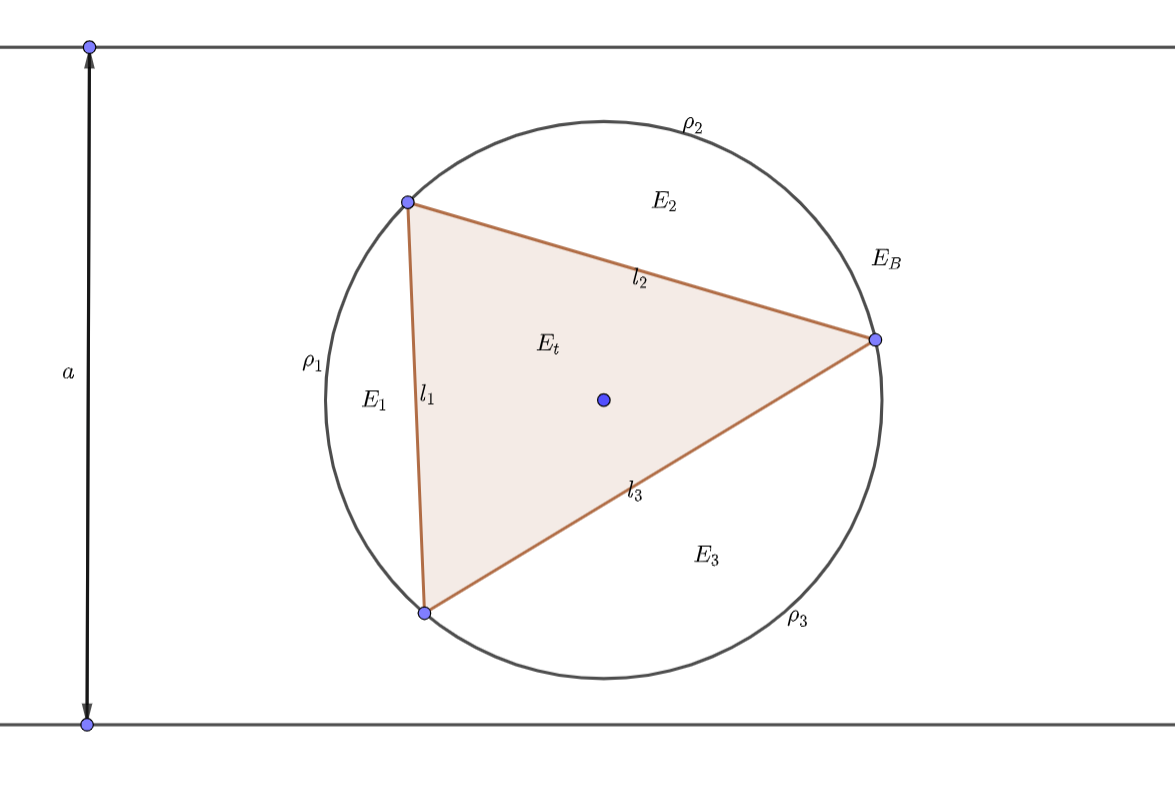
\includegraphics[width=0.8\textwidth]{figure.png}
}
% 表格模板
\renewcommand\arraystretch{0.8} % 设置表格高度为原来的0.8倍
\begin{table}[!htbp] % table标准
    \centering % 表格居中
    \begin{tabular}{p{1cm}<{\centering}p{1cm}<{\centering}p{3cm}<{\centering}p{5cm}<{\centering}} % 设置表格宽度
    %\begin{tabular}{cccc}
        \toprule
        $x_i$ & $f[x_1]$ & $f[x_i,x_{i+1}]$ & $f[x_i,x_{i+1},x_{i+2}]$ \\
        \midrule
        $x_0$ & $f(x_0)$ &                  &                          \\
        $x_0$ & $f(x_0)$ & $f'(x_0)$        &                          \\
        $x_0$ & $f(x_1)$ & $\frac{f(x_1)-f(x_0)}{x_1-x_0}$ & $\frac{f(x_1)-f(x_0)}{(x_1-x_0)^2}-\frac{f'(x_0)}{x_1-x_0}$\\
        \bottomrule
    \end{tabular}
\end{table}

\def\Log{\text{Log}} % 一个简单的宏定义
$\Log$ % 调用方法
\fi

\end{document}